\section{Vehicle Sizing} \label{section:sizing}
\subsection{Introduction}
In order to verify that our vehicle is able to satisfy the mission requirements it is vital to have an understanding of what a proposed vehicle would look like in terms of its design aspects. Factors that include propulsive, structural, aerodynamic, thermal, and many others must be considered in order to properly assess if a contending vehicle design is viable in terms of matching requirements for the mission's success.

To find a vehicle design that met the individual requirements of each subteam, a large trade study was conducted in order to develop an idea of how different factors affected each other which accumulated in the final vehicle design. Since it was determined that the propulsion system of the launch vehicle had the most direct influence in a design's ability to match the mission requirements, the figure of merit analysis started with the propulsion design.

The launch vehicle sizing process started at the highest level possible, which then became increasingly refined and filtered until the end product resulted in a few point designs that satisfactorily met mission requirements. This process revolved around a 1-degree of freedom (1DOF) mathematical model that gave time history solutions for a set of input parameters that gave insight to factors about the point design including: propellant mass required, dynamic pressure experienced, burn out time for each motor, estimated inert mass from empirical propellant mass fractions, along with others. This data was then sifted through by the aerostructures team that looked at factors such as chamber pressure and temperature history, motor dimensions, inert mass, among others, to determine if designs were good candidates for further analysis. A point design was thrown out if the inert mass required to match the specified safety factors for structural stability were not achieved, and point designs were passed forward otherwise. In the final step of this process a comprehensive 6-degree of freedom (6DOF) mathematical model study was conducted that served a dual purpose: give a refined trajectory of the vehicle’s mission, and verify the outputs from the 1-dimensional model were reasonable, which gave a sanity check to the entire process. Ultimately the 6DOF gave a finishing polish on the sizing process that gave the team confidence that the point designs that were chosen as viable candidates had a high probability of completing the mission requirements successfully.

The validity of this process in choosing viable vehicle designs that are able to satisfy all of the mission requirements is yet to be shown; however, with multiple checks and balances, namely the structural analysis fitting a particular mass budget from the 1DOF, the programs utilized were able to descope a large amount of cases to test. Also, the 1 DOF itself has been tested against known designs such as the University of Southern California’s Traveler IV in order to get a sense of the accuracy of the code, which showed very similar results to published data on those examples. It is important to note, that the 1DOF model is best at predicting and sizing a launch vehicle for nominal conditions, meaning the results of the model in terms of the total change in velocity are likely to be an under prediction of what the true value may be. This is due to the lack of off-nominal events taking place within the math simulated, but this is exactly why later in the vehicle sizing process the 6DOF is utilized, which incorporates many more factors that build a more realistic and complete prediction to the overall size of system required for a launch vehicle that meets mission requirements. It wasn't possible to start at the 6DOF for the sizing processes due to lack of particular expertise and lack of proprietary data for similar missions of this scope within our team, all of which lead to an initial starting point of having an under-defined problem. Assumptions made in the 1DOF gave a proper first step that allowed for reasonably accurate results, and the elimination of parameters that negatively affected the launch vehicle. Ultimately this process produces reasonably trustworthy results. It will be of great interest to see how well these predictions are after a launch attempt has been made to accomplish this mission. Before then, tests with the propulsion system have been planned in order to add corrective factors (accurate burn rate coefficients, true ISP efficiency, and true characteristic velocity) to the existing model which will result in an even better model prediction.


\subsection{Figure of Merit and Pareto Analysis}
The Pareto analysis, a formal technique which may be useful where many possible courses of action are competing for attention, was paired with a figure of merit analysis that allowed both methods to complement each other with the desired goal of finding how the multitude of input parameters affected the performance of a point design, and then show how the many point designs compared against each other. The figure of merit analysis generated a set of point designs for a possible launch vehicle with the parameters that were simulated summarized in \Cref{table:pareto-parameters}, with every combination of parameters being a point design tested.

\begin{table}
    \centering
    \begin{tabular}{|l|c|c|}
        \hline
        \textbf{Parameter} & \textbf{Initial Run} & \textbf{Final Run} \\ \hline
        First Stage Diameter (in) & 3.75, 4.0, 4.25, 4.5, 5.0 & 5.0, 5.25, 5.5 \\ \hline
        Second Stage Diameter (in) & 3.0, 3.5, 4.0, 4.5 & 4.0, 4.25, 4.5, 4.75 \\ \hline
        Payload Mass (kg) & 1, 3, 4, 5, 10 & 0.5 \\ \hline
        Desired Apogee Altitude (km) & 100, 125, 150, 200, 250, 300, 400 & 100, 125, 150 \\ \hline
        First Stage \(\Delta V\) Split & 35\%, 40\%, 45\%, 50\%, 55\%, 65\% & 35\%, 42.5\% \\ \hline
        Propellant Mass Fraction (\(\lambda_p\)) & \(\lambda_{p,1}\) = 0.85 \quad \(\lambda_{p,2}\) = 0.785 & \(\lambda_{p,1} = 0.7 \quad \lambda_{p,2} = 0.6\) \\ \hline
        \(I_{sp}\) Efficiency (\(\eta_{isp}\)) & 0.925 & 0.9 \\ \hline
        Total Point Designs Tested & 4200 & 72 \\ \hline
    \end{tabular}
    \caption{Summary of Pareto analysis vehicle parameters}
    \label{table:pareto-parameters}
\end{table}

Each point design was evaluated using both the 1DOF model and the genetic algorithm, with the 1DOF model being the main computational engine in the sizing process. The genetic algorithm iterated on chamber pressure profiles for the first and second stage motors in order to maximize the following characteristic evaluation function.

\begin{multline*}
    CEF = W_1 \left(1 - \frac{t_{ref}}{t_{b1} + t_{b2}}\right) + W_2 \left(\frac{m_{pl}}{m_{pl,ref}}\right) + W_3 \left(\frac{h}{h_{ref}} - 1\right) \\ 
    + W_4 \left(1 - \frac{m_{p,ref} - m_p}{m_{p,ref}}\right) + W_5 \left(1 - \frac{Q_{max,ref}}{Q_{max}}\right) + W_6 \left(1 - \left[\frac{L/D_{ref} - L/D}{L/D_{ref}}\right]^2\right)
\end{multline*}

\begin{table}
    \centering
    \begin{tabular}{cccccc}
        \(W_1\) & \(W_2\) & \(W_3\) & \(W_4\) & \(W_5\) & \(W_6\) \\ \hline
        -0.4 & 0.05 & 0.35 & -0.4 & -0.2 & 0.6
    \end{tabular}
    \vspace{0.3cm} \\
    \begin{tabular}{cccccc}
        \(t_{ref}\) & \(m_{pl,ref}\) & \(h_{ref}\) & \(m_{p,ref}\) & \(Q_{max}\) & \(L/D_{ref}\) \\ \hline
        10 sec & 5 kg & 103.57 km & 119.522 kg & 200 kPa & 19.5
    \end{tabular}
    \caption{Characteristic evaluation function weights and reference values}
    \label{table:CEF-weights-ref}
\end{table}

This characteristic evaluation function was the backbone to the Pareto analysis, which included six metrics that were chosen to best represent the performance of a potential design. The metrics chosen were: burnout times for the first and second stage (\(t_b\)), payload mass (\(m_{pl}\)), altitude at apogee (\(h\)), mass of propellant for first and second stage (\(m_p\)), maximum dynamic pressure experienced (\(Q_{max}\)), and aspect ratio for the entire vehicle (\(L/D\)). Reference values were utilized in the characteristic evaluation function in order to normalize the data as best as possible, with the values used being summarized in \Cref{table:CEF-weights-ref}. The weights chosen by our team as the values of \(W\) are designed to put emphasis on parameters deemed more impactful to the mission, and factors that have an unfavorable impact on the design have negative sign. In all, the characteristic evaluation function (CEF) is bound between -1 and 1, with a design performing the best with a score of 1. The overall distribution for point designs score of the CEF was modeled to be approximately normal. The reference values are modeled after Traveler IV, with the exception of \(t_{ref}\), \(m_{pl,ref}\), and \(Q_{max}\), which were all chosen using a point estimation for the population mean of the point designs tested in the set. Parameters such as desired altitude, payload mass, and to an extent aspect ratio are all direct input parameters to the system, whereas the rest of the values are outputs from the 1DOF model.

A plot for an example batch of point designs that have been normalized within the set are shown in \Cref{figure:pareto-points}, where the ``value'' is defined as the factors in the CEF that are positive, and the ``cost'' are the factors that are negative. The point designs that are colored in red are chosen as favorable designs since they have the best balance between the costs and value, whereas the blue labeled points have corresponding designs that may perform at the same value but with minimal cost. This method of screening was used for the initial selection process for viable point designs. This region of red dots is known as the Pareto Frontier, and the slope of the frontier shows a direct visual trade off of certain parameters of a point design to the overall performance.

\begin{figure}
    \centering
    \begin{tikzpicture}
        \begin{axis}[
            width=12cm,
            height=10cm,
            xlabel={Cost},
            ylabel={Value},
            xmin=0.7, xmax=1.0,
            ymin=0.4, ymax=1.0,
            xtick={0.7, 0.75, 0.8, 0.85, 0.9, 0.95, 1.0},
            ytick={0.4, 0.5, 0.6, 0.7, 0.8, 0.9, 1.0},
            xmajorgrids=true,
            ymajorgrids=true,
        ]
            \addplot+[
                only marks,
                red,
                mark options={draw=red}, % TODO: fix color
                scatter,
                mark=o,
                mark size=3pt,
            ]
            table{data/pareto-red.csv};
            \addplot+[
                only marks,
                mark options={draw=blue}, % TODO: fix color
                scatter,
                mark=o,
                mark size=3pt,
            ]
            table{data/pareto-blue.csv};
        \end{axis}
    \end{tikzpicture}
    \caption{Pareto analysis results scatter plot}
    \label{figure:pareto-points}
\end{figure}


The genetic algorithm used converged on a point design when the characteristic evaluation function was maximized for a given chamber pressure profile. In order to best prevent the program from settling on a local maximum, a few measures were implemented to find the solution which converged with the highest value which was the best approximation of a global maximum. The first generation that was run through the 1DOF model used a seed profile with a total of 7 ``offspring'' profiles, which were altered versions of the seed profile. Of the offspring, 4 were more conservative variations that were intended to refine the parent generation with minor adjustments, whose purpose was to converge on a local maximum of the characteristic evaluation function. The 3 other offspring profiles had much larger changes from the parent generation which are designed to bump the convergence from one local maximum to another. After the 8 profiles converged, the overall best score from the characteristic function was found, which then was chosen as the next parent seed for the following generation. This process was repeated for the designated amount of generations by the user. A visual example of this process is shown below in \Cref{figure:genetic-chamber-pressure}, where an example is shown after all schemes have been tested, and the darkened profile is selected as the parent profile for the next generation since it has the highest characteristic evaluation function score. The entire selection process is simplified in the flowchart in \Cref{figure:genetic-flowchart}.

\begin{figure}
    \centering
    \includegraphics[width=0.7\linewidth]{images/genetic-chamber-pressure}
    \caption{Example genetic algorithm run}
    \label{figure:genetic-chamber-pressure}
\end{figure}


\begin{figure}
    \centering
    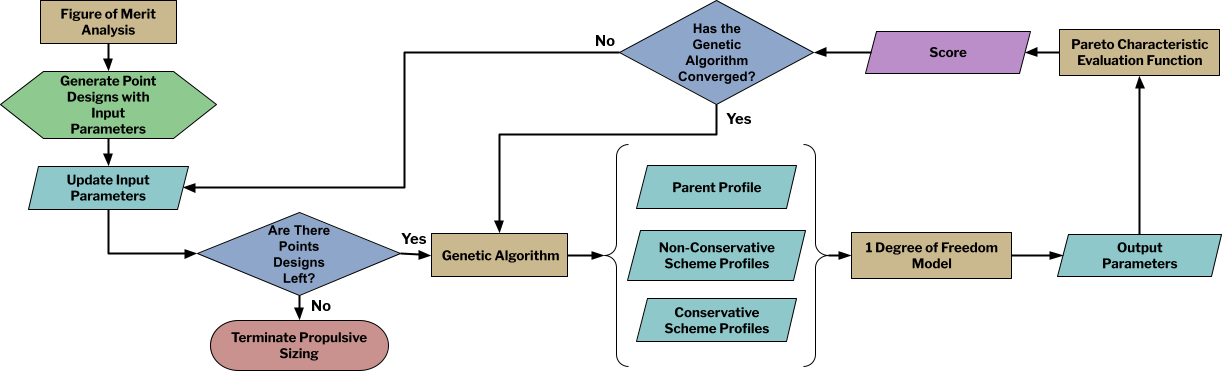
\includegraphics[width=\linewidth]{images/genetic-flowchart}
    \caption{Genetic algorithm selection process flowchart}
    \label{figure:genetic-flowchart}
\end{figure}

\subsection{One Degree of Freedom Analysis}
The 1DOF utilized in this process started by initializing a few key parameters that were held constant in each subsequent point design, which included: propellant characteristics and composition, nozzle characteristics with expansion ratio, empirical estimations for propellant mass fractions, and empirical estimation for \(I_{sp}\) efficiency.

These aspects were held to be constant with one notable exception, the propellant mass fraction estimate. Using historical data provided in Figure 3.4 of ``Rocket Propulsion'' \cite{heister-rocket-propulsion} a rough approximation was made for the propellant mass fraction, which relates the total mass of the motor to the mass of propellant. It was found later from the structures sub team, that these empirical estimations were giving values for acceptable inert masses to be less than what could be reasonably done, therefore these values had to be adjusted in order to give more inert mass to each stage so an appropriate aerostructure could be designed while fitting the designated inert mass budget. The propellant mass fraction was different for both the first and second stage, with the second stage having more inert mass accounted for, and likewise a lower inert mass fraction, due to an interstage and other factors due to the two stage nature of the vehicle.

The propellant characteristics were not adjusted due to the limitation from faculty advisors to not develop our own proprietary propellant, which would allow for individual tailoring of different traits. This limited our total selection of propellants severely, and ultimately a propellant (TS - 78) derived from published literature from NATO was  selected due to its high performance and relatively safe manufacturability. In further testing for the mission this input parameter of propellant performance will have the most direct impact on this model’s results. Currently, the propellant is modeled using NASA CEA to give motor characteristics such as: exhaust velocity, chamber temperature, motor characteristic velocity, motor ISP, and exhaust static pressure. Further tests will give improved representations of these factors.

The nozzle was held constant since it added a few extra variables to the selection process, namely throat area, exit area, and therefore expansion ratio. It was decided that these factors could be adjusted after the selection process was done if need be.

In order to properly have a solution from the 1DOF, iteration was relied on heavily to fully define the variables in the system. The main variable that was iterated upon was the mission’s total change in velocity (\(\Delta V\)), which trickled down to a few other variables. If a value for total \(\Delta V\) was estimated, then using the ideal rocket equation with the propellant mass fractions and the stage specific impulse, a value for the vehicle's mass could be found broken up between first and second stage for its inert and propellant mass. Then, once propellant mass is found for each stage, burn time per motor can be iterated upon using the mass flow rate history of each stage (derived from the chamber pressure profile, throat area, and characteristic velocity) until the total mass accumulated is equivalent to the propellant mass found with the ideal rocket equation. Following this, an atmospheric model was utilized to find aerodynamic forces on the vehicle. The flight of the vehicle was modeled using a time stepping force balance that accounted for the mass exhausted from the motor and the thrust of the motor, drag, and gravity in order to find the acceleration at a designated time. Velocity was found from the integration of acceleration, and so forth for altitude. It is key to note that all thrust was modeled to be purely axial, all aerodynamic forces were axial, and likewise with body forces from gravity. After a motor had burnt out, a coasting period was modeled, if required by the input parameters of the mission, by the same procedure just without thrust of the motor. Once separation occurred, the inert mass of the first stage was subtracted from the vehicles total mass, and the second stage followed the same procedure to find acceleration on the vehicle. This process resulted in the time history data for vehicle mass, dynamic pressure, net force, acceleration, velocity, altitude, atmospheric conditions, Mach, along with others derived from these. It is important to note that the coefficient of drag used in this model was variable and had critical Mach numbers of 0.7 and 1.3, which affected the vehicle most as it was going through Mach 1. After all of these calculations took place, the final altitude was compared to the input parameter for the desired altitude, and if the margin of error was not met, the process would be repeated with an updated delta V for the mission. Therefore this method can be thought of as a modified ideal rocket solution, since at its core it uses the ideal rocket equation to find the mass of the vehicle, but it iterates on this value to find a solution that incorporates forces other than the vehicle's thrust.


\subsection{Mass Estimation and Sizing System}
Once the propulsion team generated point designs using ranges of parameters, it was decided that further steps were necessary to visualize and analyze the selected designs, as well as generate the inputs needed to evaluate the designs using the 6 degree of freedom (6DOF) model, which will be discussed in detail in \Cref{section:6dof}. The goal of this script is to determine whether point designs can fit the propulsion analysis' inert mass requirement, while doing preliminary structural analysis to ensure these materials and geometries pass minimum safety factor requirements.


\subsubsection{General Operation and Information}
The program takes inputs from the Pareto analysis, as well as from preliminary mass and location estimates for the vehicle subsystems. Using the inputs gathered from these sources, the program then does the basic geometric layout of the rocket, generating lengths, wall thicknesses, and a design that can then be visualized with the help of tools such as OpenRocket and CAD software. The program also calculates key physical characteristics of the rocket, the center of mass and mass moment of inertia over the duration of the flight.

In order to simplify analysis, some assumptions about the rocket were made, which are covered in \Cref{table:mass-script-assumptions}. The design generated contains the position and mass of all aerostructures and internal components from both stages. These include the nosecone, the sustainer airframe, the sustainer fins, the interstage, the booster airframe, and the booster fins. Internal components include the motor, the forward closure, the nozzle, the recovery subsystem, the despin subsystem, and the avionics subsystem.

\begin{table}
    \centering
    \begin{tabular}{ | >{\raggedright}p{0.38\textwidth} | p{0.58\textwidth} | } \hline  %TODO: raggedright both cols
        \textbf{Current Assumption} & \textbf{Justification} \\ \hline
        All point designs are sub-minimum diameter & The sub-minimum design, when compared to their minimum, and other counterparts for such high powered applications, offered more benefits in mass and space saving. \\ \hline
        All point designs use metallic airframes & Sub-minimum diameter rockets require their airframes to be pressure vessels, and the team does not have the capability to make composite overwrapped pressure vessels in-house. \\ \hline
        All point designs use four fins for each stage & This assumption was made in order to perform first-order analysis; in the future, fin characteristics will be optimized by the 6DOF and prior art. \\ \hline
        All point designs have a 5:1 Von Karman nosecone & Based on prior art; for other high powered rockets the 5:1 Von Karman design was commonly used. \\ \hline
        Point designs do not have igniters, RF-transparent sections, nozzles, fasteners, or couplers & These components are a part of the detailed design, as such to reduce complexity, they were left out of the analysis. \\ \hline
        All point designs' internal rocket components' dimensions and masses are static & These components are a part of the detailed design, as such to reduce complexity, they were left static in this analysis \\ \hline
        All point designs' internal components are modeled as cylinders & In order to simplify for the first order analysis, as well as generalize for the wide range of point designs generated, the internal subteams provided us with simplified representations of their sub-systems \\ \hline
    \end{tabular}
    \caption{Mass estimation and sizing assumptions}
    \label{table:mass-script-assumptions}
\end{table}

The program also performs primary column buckling and local column buckling analysis on the sustainer airframe. This is done assuming the airframe is a fixed-free column; however this will change once the detailed design of the rocket is done. Currently this check is simply a ``sanity check'' so to speak, just as a qualifier for further analysis on each point design.


\subsubsection{Analysis}

The Pareto analysis provided the diameters of both stages, the maximum expected operating pressure (MEOP) of both motors, the mass of the motors as a function of time, the maximum drag force, and the maximum acceleration of the rocket. Additional inputs were also given in the form of material properties, and geometric properties.

The majority of the analysis was performed on the airframes, as the dimensions and stability of the airframe drive the viability of the point design.

Starting with the airframes, wall thickness of each stage was calculated using the MEOP of both motors and the thin wall hoop stress formula. The length of the motor is calculated using the propellant mass, the propellant density, and the internal diameter of the airframes. The forward closure was modeled as a uniformly loaded circular disk with clamped edges, and thickness was backsolved from the corresponding formula. The length was calculated by simply adding the length of the motor, the internals, and the bulkheads together, with some amount of room for error. The mass of the airframe and the bulkheads was calculated by calculating the volume of each and multiplying by material density. The script has three types of column buckling included, with two relevant criteria per airframe. The first, the primary buckling instability can be modeled by either the Euler or Johnson buckling formulas. The script chooses one over the other based on the slenderness ratio of the airframe and calculates the associated buckling stress. The third form of analysis is local buckling. The formula was obtained from NASA’s SP 8007 manual \cite{nasa-sp8007}, and used to calculate the critical local buckling stress.

To estimate inert masses, a simple method was used. For aerostructures, we calculated the volume of each component and multiplied by material density. For the internal components, the internal subteams were consulted on generalized masses and dimensions for each sub system that could be applied to all point designs. The motor mass was given by the Pareto analysis outputs, and is represented as a function of mass over the time duration of the flight.

The script calculates the center of mass of the rocket as a function of time, based on the motor mass time history, and was verified at the beginning and end of motor burns using OpenRocket. It also calculates the moment of inertia of the vehicle in its three principal dimensions. This was verified using SolidWorks models of point designs.


\subsubsection{Results}
After the Pareto analysis determined a significant number of viable point designs, the structures script was used to further narrow down this number. Most point designs were discarded because they could not meet inert mass requirements, while others were deemed to have motors that would be beyond our team’s manufacturing capabilities. We used the 1DOF model to simulate all designs with an altitude ceiling of 150 km, however, the 6DOF model was not ready to validate or update this parameter. 6DOF validation of these point designs will likely bring down their flight ceiling significantly, and the extra altitude provides a mass budget excess that can be used in detailed design.

The materials and geometries used in the conceptual designs are primarily outlined in \Cref{section:structures}, but the materials (aluminum, titanium, steel) were chosen for their availability, manufacturability, thermal resistance, and strength, while geometries were chosen based on prior art and manufacturability. Following the structures analysis and its simplifying assumptions, the design space determined viable point designs were found within the bounds in \Cref{table:sizing-bounds}.

\begin{table}
    \centering
    \begin{tabular}{l|c|c}
        \textbf{Variable} & \textbf{Minimum Value} & \textbf{Maximum Value} \\ \hline
        Inert Mass & 14.39 kg & 18.39 kg \\
        Propellant Mass & 28.73 kg & 34.58 kg \\
        Stage 1 Diameter & 4.5 in & 5.5 in \\
        Stage 2 Diameter & 4.0 in & 4.75 in \\
        Burn Times & 6.1 sec & 9.1 sec \\
        Inert Mass Fraction & 63\% & 67\% \\
        Delta V Split & 35\% & 42.5\% \\
        Max. Mach Number & 6.5 & 8.0
    \end{tabular}
    \caption{Design space determined by the structures sizing process}
    \label{table:sizing-bounds}
\end{table}

% TODO: hyperlink reqs
As stated in SR.4, the team wishes to have an expendable first stage. This appears viable examining prior spaceshot launches, but confirmation is needed. Sizing has established that viable point designs exist with first stages that are not recoverable, such as the 4.5 to 4 inch rocket in \Cref{figure:smaller-point}. Additionally, viable point designs exist for fully recoverable rockets, such as the 5.5 to 4.75 inch rocket in \Cref{figure:larger-point}.

\begin{figure}
    \centering
    \includegraphics[width=\textwidth]{images/4-4.5-sizing}
    \caption{The 4''-4.5'' design, shown in its expendable configuration}
    \label{figure:smaller-point}
\end{figure}

\begin{figure}
    \centering
    \includegraphics[width=\textwidth]{images/4.75-5.5-sizing}
    \caption{The 4.75''-5.5'' design, which can reasonably be flown with either a recoverable or expendable first stage}
    \label{figure:larger-point}
\end{figure}

Throughout the rest of this report the work required to arrive at this design space will be presented. All of the work requiring dimensions and masses was done with the 4 to 4.5 inch expendable rocket, as this design represents the team’s Minimum Viable Product (MVP). Once the 6DOF can evaluate the design space, then additional analysis will be performed to ensure that the assumptions and Pareto analysis still hold true.



\subsection{Trajectory Analysis Model and Statistical Methods (6DOF)} \label{section:6dof}
